\documentclass{beamer}

\usepackage[english]{babel}
\usepackage[latin1]{inputenc}
\usepackage{amsmath,amsfonts,amssymb}
%\usepackage[dvips]{graphicx}
\usepackage{graphics}
\usepackage{sidecap}
\usepackage{floatrow}
\usepackage{pifont}
\newcommand{\tick}{\ding{52}}
\newcommand{\emptyline}{\vspace{\baselineskip}}
\definecolor{links}{HTML}{2A1B81}
\hypersetup{colorlinks,linkcolor=,urlcolor=links}
\newcommand{\tabitem}{% To center items in itemize like way
  \usebeamertemplate{itemize item[]}\hspace*{\labelsep}}
\newcommand{\ra}{\rightarrow}
\newcommand{\zenodo}{\href{http://dx.doi.org/10.5281/zenodo.61771}{Zenodo}}
\newcommand\todo[1]{\color{red}#1\color{black}}
%\usepackage[colorlinks = true,linkcolor = blue,urlcolor  = blue,citecolor = blue,anchorcolor = blue]{hyperref}
%\usepackage{epstopdf}
%\usetheme{Copenhagen}
%\usecolortheme{beaver}
\usetheme{boxes}
\usecolortheme{default}
%\useoutertheme{infolines}
%\setbeamercovered{transparent}
\beamertemplatenavigationsymbolsempty
%\setbeamertemplate{footline}[frame number]
\setbeamercolor{block body}{bg=white}
\setbeamercolor{block head}{bg=white}
\setbeamercolor{item}{fg=gray}
%\setbeamertemplate{caption}[numbered]
\defbeamertemplate*{footline}{shadow theme}
{%
  \leavevmode%
\  \hbox{
%\begin{beamercolorbox}[wd=.5\paperwidth,ht=4ex,dp=1.125ex,leftskip=.3cm plus1fil,rightskip=.3cm]{author in head/foot}%
%    \usebeamerfont{author in head/foot}\insertshortauthor
%  \end{beamercolorbox}%
%  \begin{beamercolorbox}[wd=.5\paperwidth,ht=4ex,dp=1.125ex,leftskip=.3cm,rightskip=.3cm plus1fil]{title in head/foot}%
  \begin{beamercolorbox}[wd=\paperwidth,ht=4ex,dp=1.125ex,leftskip=.3cm,rightskip=.3cm plus1fil]{white}%
    \usebeamerfont{title in head/foot}\hfill\insertframenumber\,/\,\inserttotalframenumber%
  \end{beamercolorbox}}%
  \vskip0pt%
}
\title[denbi]{de.NBI and its Galaxy interface for RNA folding}
%\subtitle{}

\author[J. Fallmann, J. Engelhardt ,Bioinf Leipzig]{
	J\"org Fallmann, Jan Engelhardt
}
\institute[IfI]{Institute for Bioinformatics\\University of Leipzig}
\date{\today}

\begin{document}
\titlepage

\frame{
  \section{Downloads}
  
  You can download the pdfs you will need today here
  \href{http://www.bioinf.uni-leipzig.de/~fall/RNA\_folding\_workshop-presentation.pdf}{http://www.bioinf.uni-leipzig.de/$\sim$fall/RNA\_folding\_workshop-presentation.pdf}\\
  \href{http://www.bioinf.uni-leipzig.de/~fall/Exercises.pdf}{http://www.bioinf.uni-leipzig.de/$\sim$fall/Exercises.pdf}
}
\section{Vienna RNA package}
\subsection{The Program \texttt{RNAfold}}
%Our first task will be to do a structure prediction using
%\texttt{RNAfold}. This should get you familiar with the input and output
%format as well as the graphical output produced. \texttt{RNAfold} reads
%RNA sequences from \emph{stdin}, calculates their minimum free energy
%(\texttt{MFE}) structure, prints the \texttt{MFE} structure in
%dot-bracket notation and its free energy to \emph{stdout}. If the
%\texttt{-\/-partfunc} option is set it also computes the partition function, the
%base pairing probability matrix and additionally prints the free energy
%of the thermodynamic ensemble, the frequency of the \texttt{MFE}
%structure in the ensemble and the ensemble diversity \todo{to \emph{stdout}}.
%Another useful option is the \texttt{-\/-MEA} option, which also shows
%the maximum expected accuracy, but remember that this also needs more
%CPU time than without \texttt{-\/-MEA}.

\frame{
\textbf{Goal}:
Use \texttt{RNAfold} to do a simple structure prediction.

\begin{itemize}
\item Upload the file \texttt{rna.fa} into your Galaxy session.
\item Start \texttt{RNAfold} with standard parameters
\item Look into the output
\end{itemize}
}

\frame{
  \begin{itemize}
  \item CUACGGCGCGGCGCCCUUGGCGA
  \item $...........((((...)))).$ ( -5.00)
  \end{itemize}
  \vskip20pt
  \center
  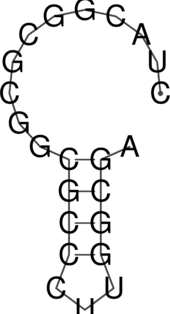
\includegraphics[scale=.4]{Figs/test_ss.png} 
}

\frame{
\textbf{Goal}:
Use \texttt{RNAfold} to do a structure prediction using the partition function

%\todo{--partfunc and --MEA can not be used at the same time}

\begin{itemize}
\item Start \texttt{RNAfold} using -\/-partfunc
\item Look into the output
\end{itemize}
}

\frame{
  \begin{itemize}
  \item CUACGGCGCGGCGCCCUUGGCGA
  \item MFE: ...........((((...)))). ( -5.00)
  \item PF: $....\{,\{\{...||||...)\}\}\}.$ [ -5.72]
  \end{itemize}

  The partition function is a rough measure for the well-definedness of
  the MFE structure. The third line shows a condensed representation
  of the pair probabilities of each nucleotide, similar to the
  dot-bracket notation, followed by the ensemble free energy ($-kT*ln(Z)$) in kcal/mol
}

\frame{
  \begin{itemize}
  \item CUACGGCGCGGCGCCCUUGGCGA
  \item MFE: ...........((((...)))). ( -5.00)
  \item PF: $....\{,\{\{...||||...)\}\}\}.$ [ -5.72]
  \item CS: $.......................$ \{ 0.00 d=4.66 \}
  \item MEA: $......((...))((...))...$ \{ 2.90 MEA=14.79 \}
  \item frequency of mfe structure in ensemble 0.311796; ensemble diversity 6.36
  \end{itemize}
  Pseudo bracket notation:\\ Here, the usual '(', ')', '.', represent
  bases with a strong preference (more than 2/3) to pair upstream
  (with a partner further 3'), pair down-stream, or not pair,
  respectively. '{', '}', and ',' are just weaker version of the above
  and '$|$' represents a base that is mostly paired but has pairing
  partners both upstream and downstream. In this case open and closed
  brackets need not match up.
  
}

\frame{
  \center
  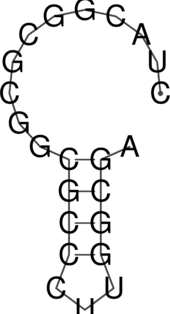
\includegraphics[scale=.45]{Figs/test_ss.png} 
  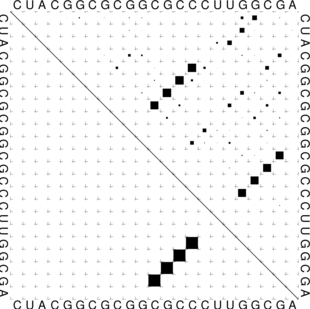
\includegraphics[scale=.45]{Figs/test_dp.png} 
}

\frame{
\textbf{Goal}:
Use SHAPE-directed \texttt{RNAfold} to do a structure prediction
%
%%\todo{problem with shape files}
%
\begin{itemize}
\item Upload the file \texttt{rna.simple.shape} into your Galaxy session.
\item Start RNAfold using the shape file and  -\-shapeMethod=D
\item Look into the output
\end{itemize}
}

%\subsection{The Program \texttt{RNApvmin}}
%\frame{
%\textbf{Goal}:
%Use \texttt{RNApvmin} to assist the SHAPE directed \texttt{RNAfold}.
%
%\todo{not tested}

%\begin{itemize}
%\item Use \texttt{RNApvmin} with the rna.shape file and rna.seq to create a vector.csv
%\item Start \texttt{RNAfold} using the vector.csv as shape file and  -\/-shapeMethod=W
%\item Compare the output with the other shape method
%\end{itemize}
%}

\subsection{The Program \texttt{RNAcofold}}
\frame{
\textbf{Goal}:
Use \texttt{RNAcofold} to predict the cofolding of two sequences.

%\todo{--partfunc does not make an rna structure eps, without
%  --partfunc two eps outputs are generated, one is empty}

\begin{itemize}
\item Upload the file \texttt{cofold.txt} into your Galaxy session. (Look at it)
\item Start RNAcofold using cofold.txt with the -\/-partfunc option
\item Look at the output.
\end{itemize}
}

\frame{
  \begin{itemize}
  \item GCGCUUCGCCGCGCGCC\&GCGCUUCGCCGCGCGCA
  \item ((((..((..((((...\&))))..))..))))... (-17.70)
  \item ((((..{(,.((((,,.\&))))..}),.)))),,. [-18.26]
  \item frequency of mfe structure in ensemble 0.401754 , delta G binding= -3.95
  \end{itemize}
}

\frame{
  \center
  
\includegraphics[scale=.45]{Figs/t_ss.png} 
  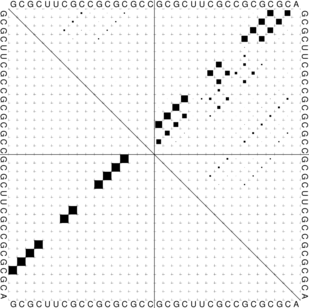
\includegraphics[scale=.45]{Figs/t_dp.png}

  Cofold can use concentrations of molecules for duplex prediction, but this is slow for longer sequences.
}

\subsection{The Program \texttt{RNAduplex}}
\frame{
\textbf{Goal}:
Use \texttt{RNAduplex} to predict \textit{only} intermolecular base pairs of two sequences.

\begin{itemize}
\item Upload the file \texttt{duplex.txt} into your Galaxy session. (Look at it)
\item Start RNAduplex using duplex.txt with standard parameter
\item Look at the output.
\end{itemize}

RNAduplex does not use concentrations and neglects intramolecular interactions, faster but less reliable, good prefilter.

}

\frame{
\textbf{Goal}:
Use \texttt{RNAup} to test the \texttt{RNAduplex} result.

\begin{itemize}
\item Start RNAup using duplex.txt with -\/-include\_both
\item Look at the output and compare it with the RNAduplex result.
\end{itemize}

RNAup is also taking intramolecular interactions into account.

}

\frame{
\textbf{Goal}:
Use \texttt{RNAalifold} to predict the consensus structure

\begin{itemize}
\item Upload the clustal file \texttt{alifold.aln} into your Galaxy session. 
\item Edit the data type of alifold.aln to 'clustal'
\item Use RNAalifold with the alifold.aln and -\/-partfunc (Calculate partition function: 1)
\item (Download the output) and look at it
\item \texttt{Bonus}: Fold the sequences (alifold.fa) individually (RNAfold) and compare the results.
\end{itemize}
}


\frame{
\textbf{Goal}:
Use \texttt{RNAalifold} to predict \textit{and visualize} the consensus structure

\begin{itemize}
\item Use RNAalifold with alifold.aln and -\/-color and -\/-aln
\item (Download the output) and look at it
\end{itemize}

}

\frame{
  \center
  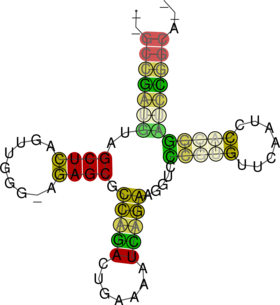
\includegraphics[scale=.45]{Figs/alirna.png} 

  RNAalifold uses covariance information from sequence alignment to predict a consensus structure.

}

\frame{
\textbf{Goal}:
Use \texttt{RNAcode} to predict coding sequences in a MAF alignment.

\begin{itemize}
\item Upload the file \texttt{oskar.27way.rnacode.maf} into your Galaxy session.
\item (Change its data type to maf)
\item Use RNAcode with the maf file, --cutoff 0.05, --best\_region, --best\_hit, with GTF output
\item (Download the output) and look at it
\end{itemize}
}

\frame{
\textbf{Goal}:
Use \texttt{RNAz} 

%\todo{rnaz output is treated as fasta file and inmportant information is missing}

\begin{itemize}
\item Upload the file \texttt{oskar.27way.rnaz.maf} into your Galaxy session.
\item Use RNAz with the maf file
\item (Download the output) and look at it
\end{itemize}
}

\end{document}

%%% Example environments
\frametitle{}
       \begin{itemize}
         \item 1
         \item 2
       \end{itemize}     
  \begin{columns}[T]
    \begin{column}{.25\paperwidth}
     \begin{block}{}
\vskip-18pt
        %\includegraphics[scale=.2]{figures/TTP.eps}
     \end{block}
    \end{column}
    \begin{column}{.5\paperwidth}
      \begin{block}{}
\vskip10pt 3
      \end{block}
    \end{column}
  \end{columns}
\begin{center}
\vskip-8pt
  How?
\end{center}
